\section{Preliminary Findings}
 
To develop a conceptual framework for improving tool recommendations, we first examined existing methods for making tool recommendations.

\subsection{[\peer] ``How Software Users Recommend Tools to Each Other" (Completed, Spring 2017)}

\subsubsection{Motivation:}

% \subsection{Peer Interactions}

% What are peer interactions?
While there are many automated technical approaches and RSSEs for making recommendations to software engineers, prior work shows that suggestions from humans is still the best. Murphy-Hill and colleagues compared interactions between peers to five other methods for tool recommendations: Tool Encounters; Tutorials; Written Descriptions; Twitter or RSS Feeds; and Discussion Threads. They found that \textit{peer interactions}, or the process of users discovering tools from their peers during normal work activities, are the most effective mode of tool discovery for software engineers~\cite{Murphy-Hill2011PeerInteraction,Murphy-Hill2015HowDoUsers}. Similarly, Xiao and colleagues found that most developers discovered security tools through recommendations from coworkers~\cite{Xiao2014Security}. Furthermore, research shows peer learning is effective for increasing knowledge and adopting ideas in areas of software engineering, pair programming~\cite{WilliamsPairProgramming}. We explored what characteristics of peer interactions make them effective for tool adoption to provide insight into improving automated recommendation approaches~\cite{VLHCC}. These results are presented in Section 4.

\subsubsection{Peer Interactions:}

% Researchers have examined a wide variety of methods to increase tool adoption among software developers. Murphy-Hill examined various modes of tool discovery and found that \textit{peer interactions}, or the process of discovering tools from colleagues during normal work activities, are the most effective way software engineers learn about new tools~\cite{Murphy-Hill2015HowDoUsers,Murphy-Hill2011PeerInteraction}. However, there is limited research exploring exactly why human-to-human recommendations are so effective. In this project, we observed peer interactions to gain a better understanding of what makes recommendations between users an effective way to learn about new tools. Our results present implications for improving tool recommendation approaches and provide a foundation for this work for creating digital nudges and designing automated systems for suggesting software engineering tools and actions to developers.

\subsubsection{Research Question:}

\begin{itemize}
  \item[\textbf{RQ}] What characteristics of peer interactions make recommendations effective?
\end{itemize}

\subsubsection{Methodology:}

To evaluate peer interactions in this study, we designed a mixed-methods approach to collect qualitative and quantitative data collected from observing participants.

\paragraph{Participants.} To evaluate the effectiveness of peer interactions, we observed pairs of software users completing data analysis tasks. We recruited undergraduate and graduate students at North Carolina State University as well as professional analysts from the NC State Laboratory for Analytic Sciences\footnote{https://ncsu-las.org/} (LAS) to participate in our study. We observed 13 pairs of participants in total, seven student pairs and six LAS pairs. We requested participants complete a questionnaire survey to collect demographic information and conducted a semi-structured post-interview to gather more data for our results. 

\paragraph{Tasks.} The study tasks involved analyzing data from the Titanic shipwreck and solving problems based on the Kaggle data science competition~\cite{KaggleTitanic}. For our study we did not examine for correctness in task completion, but were interested in how participants recommended tools to each other to solve the tasks. We allowed participants to use the software of their choice for the tasks, but prohibited Internet use to prevent participants form looking up information about the tasks or how to use tools during the study. More information on the tasks, datasets, and study materials are publicly available online.\footnote{http://www4.ncsu.edu/~dcbrow10/files/peer-interaction/study.html} For each session, we screen and voice recorded the participants while they completed the tasks. Similar to pair programming, in this study we refer to the driver as the participant actively operating the keyboard and mouse while the navigator observes and works with the driver~\cite{WilliamsPairProgramming}.

\paragraph{Study Design.} We explored five characteristics of peer interactions to determine what makes them effective: Politeness, Persuasiveness, Receptiveness, Time Pressure, and Tool Observability. These characteristics were motivated from research in psychology and qualitative results from Murphy-Hill's prior work on peer interactions. We used psychology research to compile a list of criteria for politeness~\cite{LeechPolite}, persuasiveness~\cite{ShenPersuasive}, and receptiveness~\cite{FoggPersuasiveTech}. We searched for statements made by participants about the time and pace of the session to observe time pressure. Tool observability refers to whether or not a tool is visible through a user interface. 

To observe these characteristics in peer interactions, we developed a model for analyzing recommendations based on recommendations between peers shown in Figure~\ref{fig:rec-model}. First, both peers analyze the task and develop strategies for solving it. Then the driver begins executing their method to accomplish the task, when the navigator notices a mismatch between their method and the driver's method. This could be observing a task-solving strategy they are unfamiliar with or an inefficient strategy they can improve upon. Finally, a dialogue occurs between the peers where the navigator asks about the driver's strategy or provides the driver with a more efficient method to solve the problem.

\paragraph{Data Analysis.} To measure effectiveness, each software tool recommendation between participants was categorized as \textit{effective}, \textit{ineffective}, and \textit{unknown}. For effective recommendations, the recommendee used a tool after it was suggested by their partner for the remainder of their session for a majority of the opportunities it was applicable. For ineffective recommendations, the recommendee mostly ignored a tool recommended by their partner when they had a chance to utilize it in the study. Finally, unknown recommendations were the case where there was not another opportunity for the recommendee to use a suggested tool for the rest of their study session.

Two researchers independently viewed recordings of each session to note instances of tool recommendations and categorize the peer interactions based on the criteria defined for each of these characteristics, before coming together to discuss. We calculated our inter-rater agreement using Cohen's Kappa for politeness ($\kappa$ = 0.50), persuasiveness ($\kappa$ = 0.28), and 
receptiveness ($\kappa$ = 0.51).


%%% Maybe be too much info
\noindent
\begin{figure}
\centering
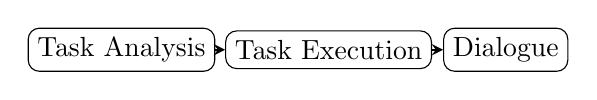
\begin{tikzpicture}
\node (task) [rectangle, rounded corners,text centered, draw=black,node distance=2.5cm] {Task Analysis};
\node (exec) [rectangle, rounded corners,text centered, draw=black, right of=task, node distance=2.63cm] {Task Execution};
\node (dial) [rectangle, rounded corners,text centered, draw=black, right of=exec,node distance=2.25cm] {Dialogue};
\tikzstyle{arrow} = [thick,->,>=stealth]
\draw [arrow] (task) -- (exec);
\draw [arrow] (exec) -- (dial);
\end{tikzpicture}
\caption{Recommendation Model}
\label{fig:rec-model}
\end{figure}

\subsubsection{Results:}

These results were published in the 2017 Visual Languages and Human-Centric Computing (VL/HCC) conference~\cite{VLHCC}. In total we discovered 142 total recommendations between participants in out study: 71 effective; 35 ineffective; and 36 unknown. Out of the five peer interaction characteristics we analyzed, \textit{receptiveness} was the only characteristic that significantly impacted the outcome of a tool recommendation between peers (Wilcoxon, \textit{p} = 0.0002). Our results show that tool recommendations targeting the receptivity of users when making suggestions are more effective than those that don't. In this study, we defined receptiveness based on prior work by Fogg on designing persuasive technology~\cite{FoggPersuasive}. There were two criteria for observing receptiveness: \textit{\textbf{Demonstrate Desire}} and \textit{\textbf{Familiarity}}. In future work, we plan to design and evaluate automated recommendation approaches that prioritize receptiveness to make more effective suggestions to developers.

\subsection{[\tele] ``Sorry to Bother You: Designing Bots for
Effective Recommendations" (Completed, Spring 2019)}

\subsubsection{Motivation:}

While recommendations between humans are the most effective, they are not always be the most practical way to increase awareness of useful development tools. For example, even though Murphy-Hill and colleagues discovered that developers prefer peer interactions for tool discovery, they also found that peer interactions occur less frequently in the workplace~\cite{Murphy-Hill2011PeerInteraction}. As development teams become larger and more distributed, effective automated recommendations are necessary to improve tool adoption among software engineers.

Bots are useful for automating tasks and improving user effectiveness and efficiency~\cite{StoreyBots}. However, they can also be inconvenient during interactions with humans. To better understand the impact of bots on human behavior and identify a baseline for automated recommendations, we evaluated making development tool recommendations to software engineers using our \telemarketer. In this study, we gathered feedback from developers receiving recommendations from a naive version of \TOOL to better understand user reactions to automated recommendations and to set the groundwork for designing better solutions for future approaches to improve the effectiveness of automated suggestions from bots.

\subsubsection{\telemarketer:}

To evaluate a basic design for making automated recommendations, we developed \telemarketer. This approach behaves similar to a telemarketer in that it ``calls" users to deliver a static message that never deviates from the script and lacks the social context necessary to adjust messages and respond to questions. \telemarketer sends developers a generic message with information about the tool, displays a generic code snippet with a common programming error, and provides sample output from the tool. This is not the best approach for making recommendations, however we implemented this simple design to better understand how bots influence human behavior and how developers respond to automated recommendations. With this naive design, we identified a baseline to motivate integrating concepts from nudge theory into future automated recommendation designs. 

% The \telemarketer approach has high actionability and spatial locality, but low temporal locality.  Generating pull requests for developers allows for high actionability in recommendations. Developers can choose to merge the pull request recommending the tool into the source code, close the pull request to reject the recommendation, or ignore the request. For spatial locality, pull requests are made on the projects and update the code base to add tools to build configuration files. However, this approach has low temporal locality due to the fact recommendations are made randomly on projects without considering time or recent changes. 

\subsubsection{Methodology:}

\paragraph{Implementation.} To evaluate our \telemarketer approach, we implemented \TOOL to make basic tool recommendations to GitHub developers. \TOOL integrates this simple approach by making generic recommendations as automated pull requests on repositories. On GitHub, pull requests are the preferred method to propose changes to repositories\footnote{https://help.github.com/articles/about-pull-requests/}. Automated pull requests have also been used by bots in related work, for example by Mirhosseini and colleagues to encourage GitHub developers to upgrade out-of-date dependencies for repositories~\cite{SamUgrade}. Figure~\ref{fig:tele} presents a screenshot of a recommendation from our system for this study. In this experiment, \TOOL recommendations provided basic information about the Java static analysis tool \EP  (Fig.~\ref{fig:tele}.A). It also presents a simple coding error in Java, using ``\texttt{==}" to evaluate string equality instead of the \texttt{String.equals()} method (Fig.~\ref{fig:tele}.B1), and the corresponding output from \EP reporting a \texttt{StringEquality} error\footnote{http://errorprone.info/bugpattern/StringEquality} (Fig.~\ref{fig:tele}.B2). To make recommendations, \TOOL automatically adds the \EP plugin to Maven\footnote{http://maven.apache.org}, to Project Object Model (\textit{pom.xml}) configuration files and created automated pull requests with the changes. An example pull request from our system using the \telemarketer can be found here.\footnote{https://github.com/CSC-326/JSPDemo/pull/2}

\begin{figure}
\centering
	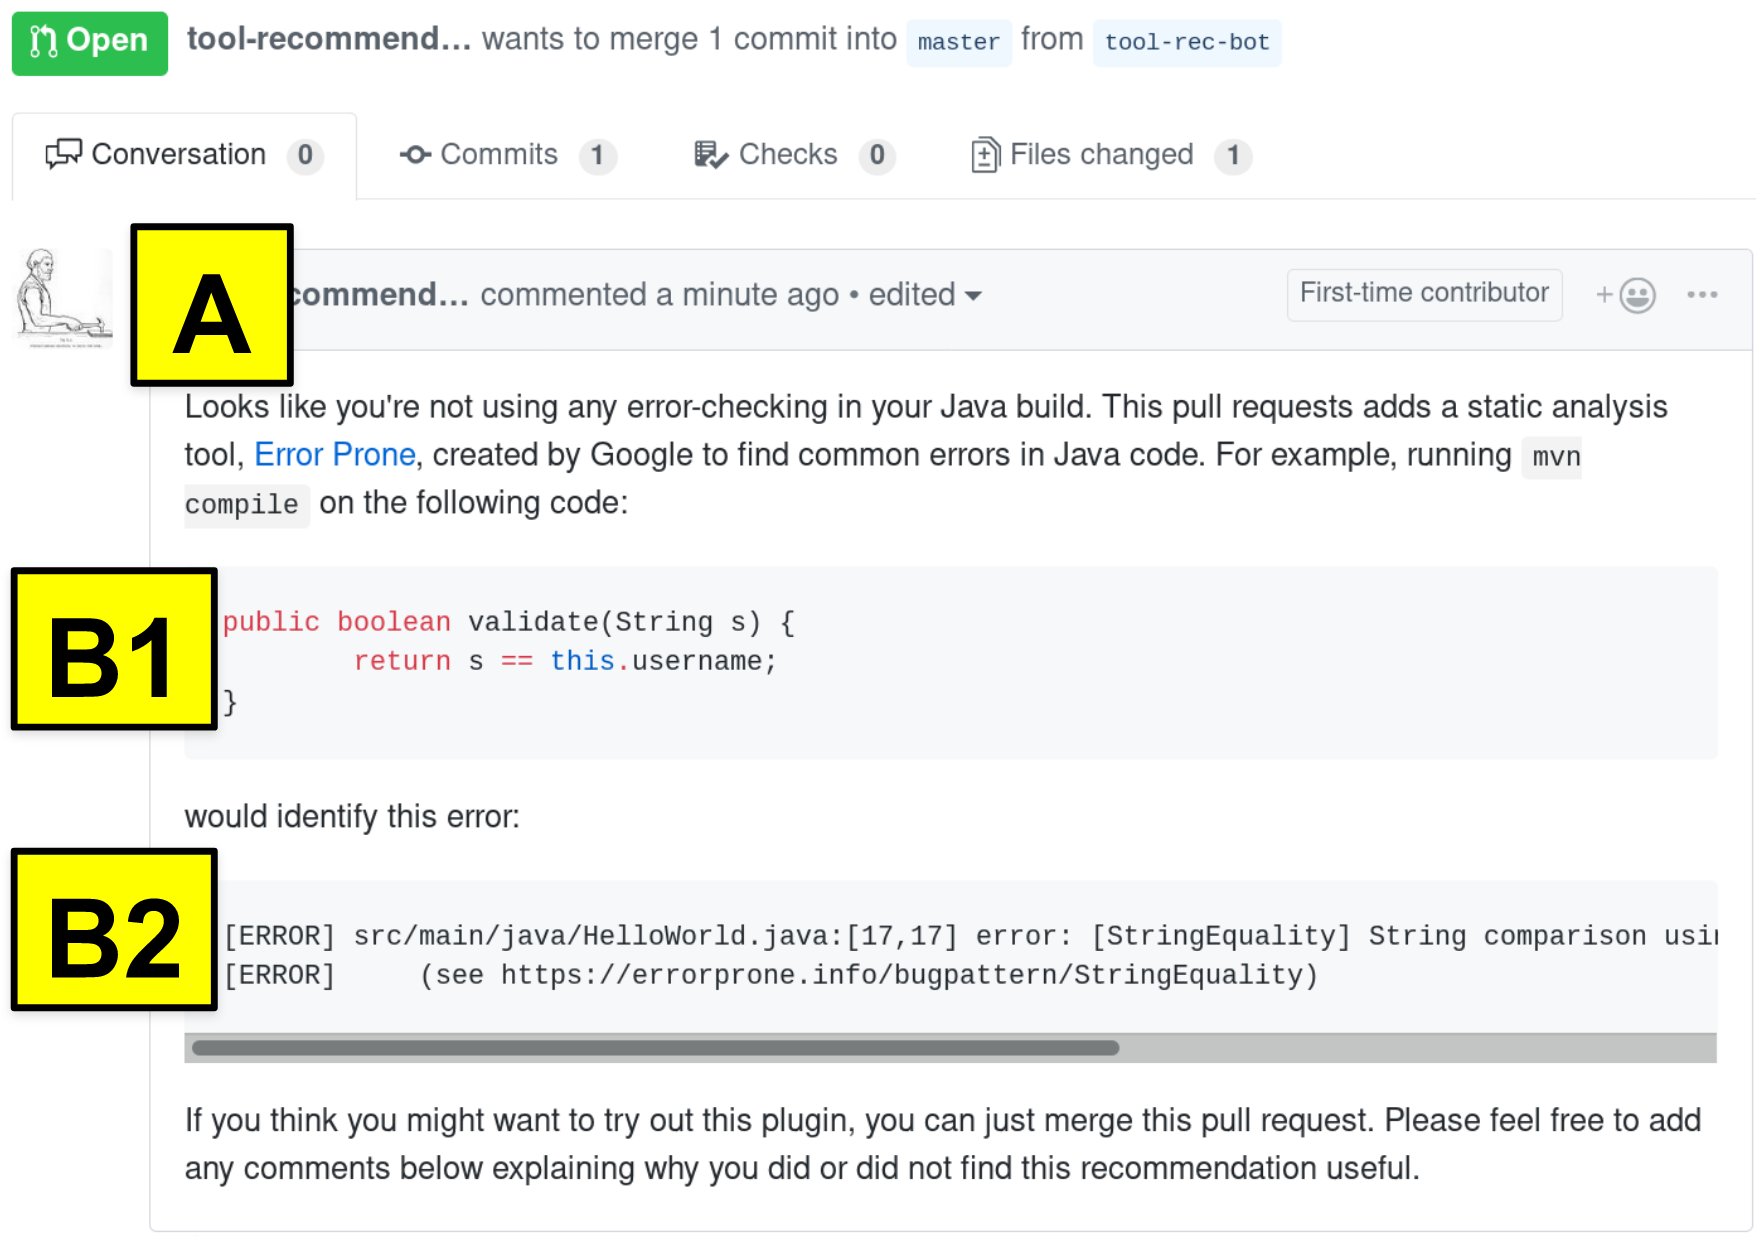
\includegraphics[width=0.5\textwidth]{images/pull.png}
	\caption{Example \telemarketer recommendation}	
	\label{fig:tele} 
\end{figure}

\paragraph{Projects.}

We sampled public open source software repositories on GitHub used in the evaluation for Repairnator\footnote{https://github.com/Spirals-Team/repairnator/blob/master/resources/data/results-buildtool.csv}~\cite{Repairnator}, an automated program repair bot~\cite{Repairnator}. Our evaluation sought to determine the effectiveness of our \telemarketer recommendation approach to developers working on real-world software applications. The projects we selected projects were required to be primarily written in Java 8 or higher, successfully validate and compile with Maven, and not already include \EP in the build configuration. Based on these criteria, we identified 52 projects for our experiment that received an automated pull request recommendation from \TOOL. The list of projects for this evaluation is available online\footnote{https://go.ncsu.edu/botse-projects}.

\paragraph{Data Analysis.}

To observe the effectiveness of \telemarketer, we categorized automated recommendations from \TOOL as \textit{effective} or \textit{ineffective} based on the status of pull requests. Effective recommendations were merged pull requests, while ineffective recommendations were closed or left open by developers. We observed recommendations for a week to gather quantitative and qualitative data. We measured rate of effectiveness by calculating the percentage of merged pull requests. Additionally, we encouraged developers to provide feedback on whether they found the recommendation useful or not and analyzed comments on the pull requests comments from GitHub users. 

\subsubsection{Results:} 

We found that bots with basic approaches are not effective for influencing human behavior. In our evaluation, \telemarketer only made two successful recommendations out of 52 (4\%). We also observed 10 closed pull requests and 40 recommendations with no response from developers. While this approach has high actionability for users, most developers provided negative feedback in comments and by closing or ignoring pull requests. According to developer responses, the main drawbacks to the \telemarketer are a lack of \textit{\textbf{social context}} and interfering with \textit{\textbf{developer workflow}}, i.e., by breaking project builds. Based on these findings, we propose using concepts from nudge theory improve social context and developer workflow for automated suggestions to software developers. The results of this research have been accepted for publication at the 1st International Workshop on Bots in Software Engineering\footnote{https://botse.github.io/} at ICSE 2019~\cite{Bots}.

